\par Evidence for the exclusive Higgs boson was searched for in events in which the Standard Model 
Higgs boson decays to a pair of \Wpm\ bosons, which in turn decay leptonically. This leptonic 
decay includes $\tau$ leptons, but only those that decay leptonically. Effectively, the final state leptons 
are electrons and muons. The topology for this decay channel is therefore 

\begin{equation}
gg\to[H]\to[\Wplus][\Wminus]\to[l][l][\met],
\label{eq:topExclH}
\end{equation} 
 
where $l$ represents the leptons: $\mu$ or $e$. 

\par The topology in Equation~\ref{eq:topExclH} is the same topology used to search for the inclusive 
Higgs boson in Ref~\cite{ATLAS:2014aga}. The event selection criteria in this analysis mimics the same 
selection criteria in Ref~\cite{ATLAS:2014aga}. Here, the flavor of the two leptons was required to be 
opposite to suppress backgrounds from \Zee\ or \Zmm\ events. Signal events were therefore required to have only 
two leptons of different flavor satisfying the selection criteria outlined in Section~\ref{sec:objExclH}.
The impact parameters of the lepton tracks with respect to the beamline in the ID, $z_0$, 
were required to be less than 1.0~mm from each other. In addition, the charges of the two leptons 
were required to be opposite because the SM Higgs boson is neutral to electromagnetic charge.  

\par Of the two leptons in signal events, the one with the largest \pt is referred to as the {\it leading} 
lepton, otherwise it is the {\it sub-leading} lepton. The leading lepton was required to have at least 
25~\GeV\ in \pt\ and the sub-leading lepton was required to have at least 15~\GeV\ in \pt. Moreover, the mass 
of the di-lepton system, \mll, was required to be at least 10~\GeV. 
This selection is referred to as the {\it pre-selection}.
Recalling that only different flavor lepton 
pairs are considered, the symbol \mll\ is used interchangeably with \memu\ to represent the transverse 
mass of the di-lepton system.

\begin{figure}[!h]
\begin{subfigure}{0.5\textwidth}
   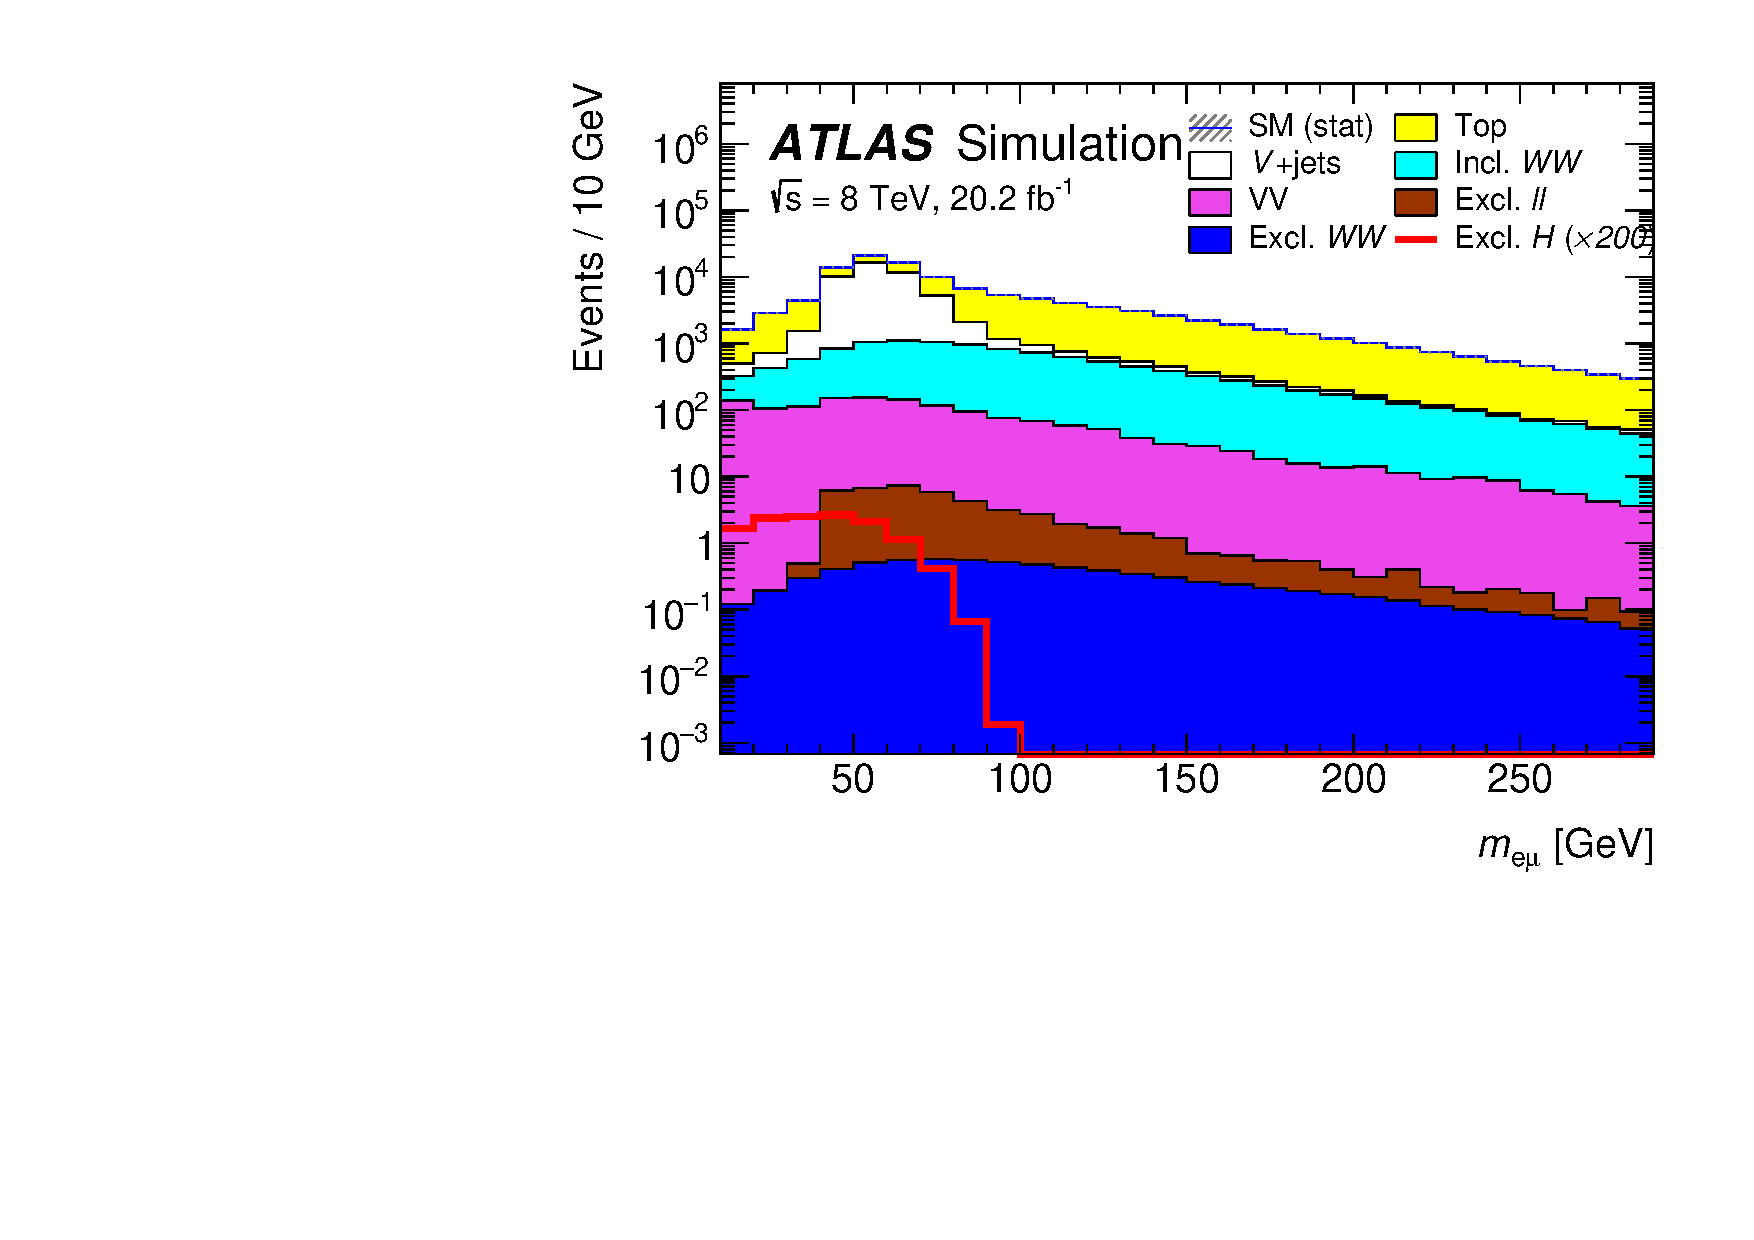
\includegraphics[width=\textwidth]{figures/emme-CutMll-Mll-log.pdf}
\end{subfigure}
\begin{subfigure}{0.5\textwidth}
   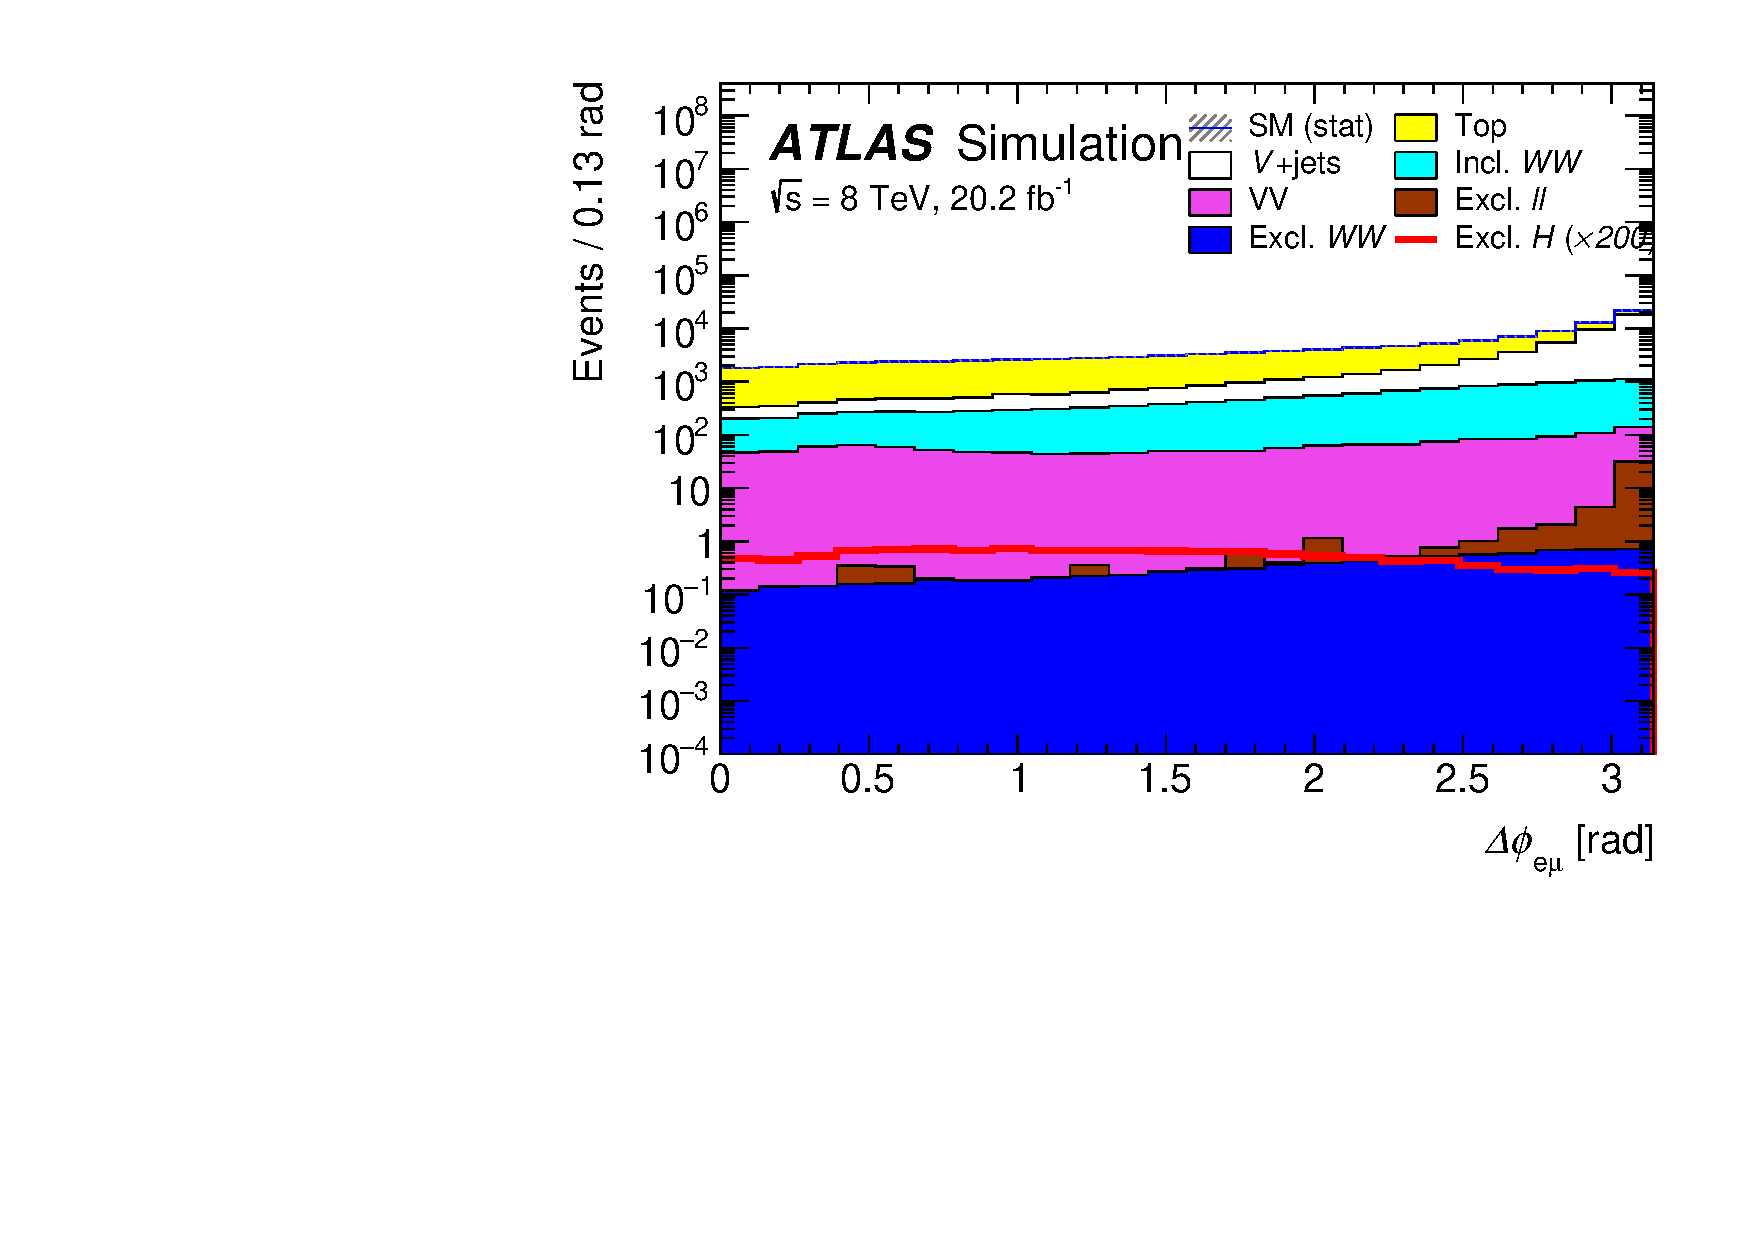
\includegraphics[width=\textwidth]{figures/emme-CutMll-DPhill-log.pdf}
\end{subfigure} 
\begin{subfigure}{0.5\textwidth}
   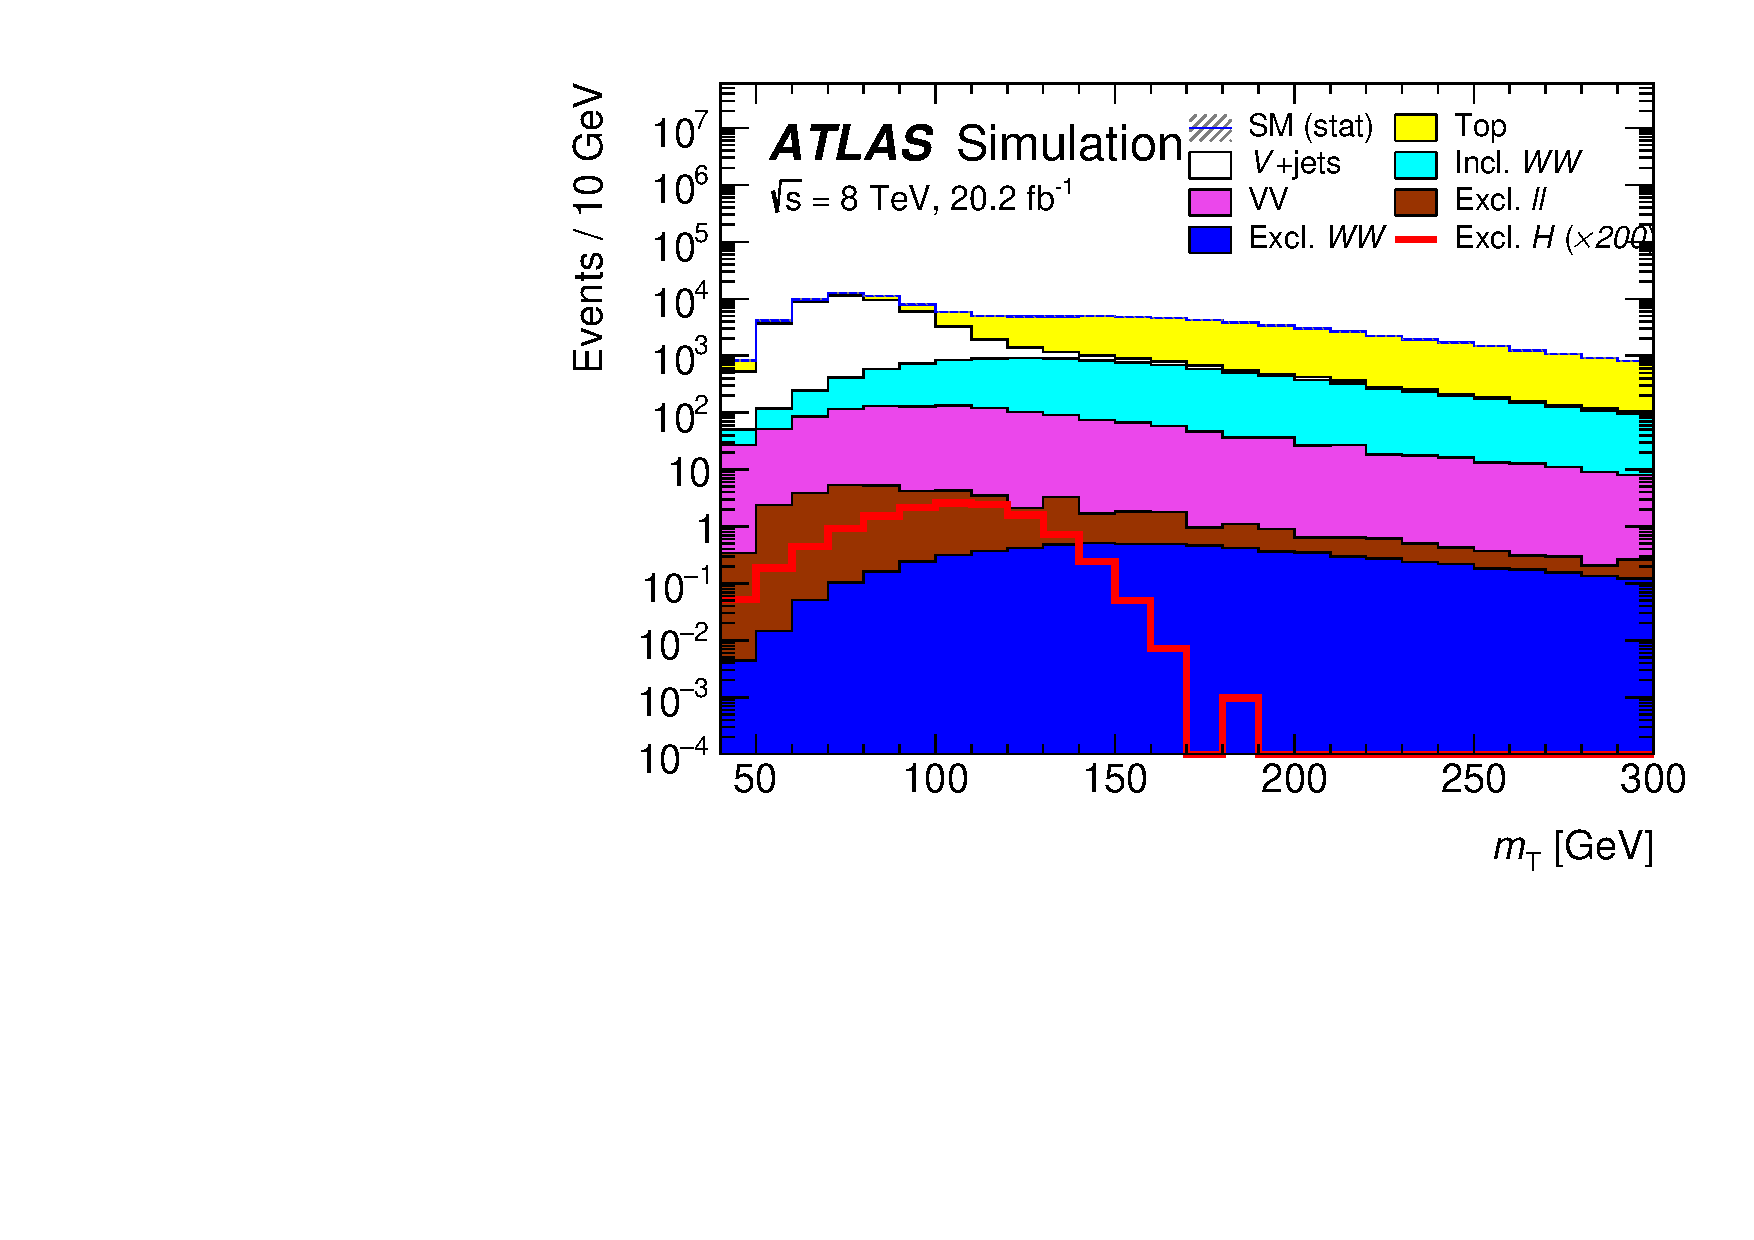
\includegraphics[width=\textwidth]{figures/emme-CutMll-MT-log.pdf}
\end{subfigure} 
\begin{subfigure}{0.5\textwidth}
   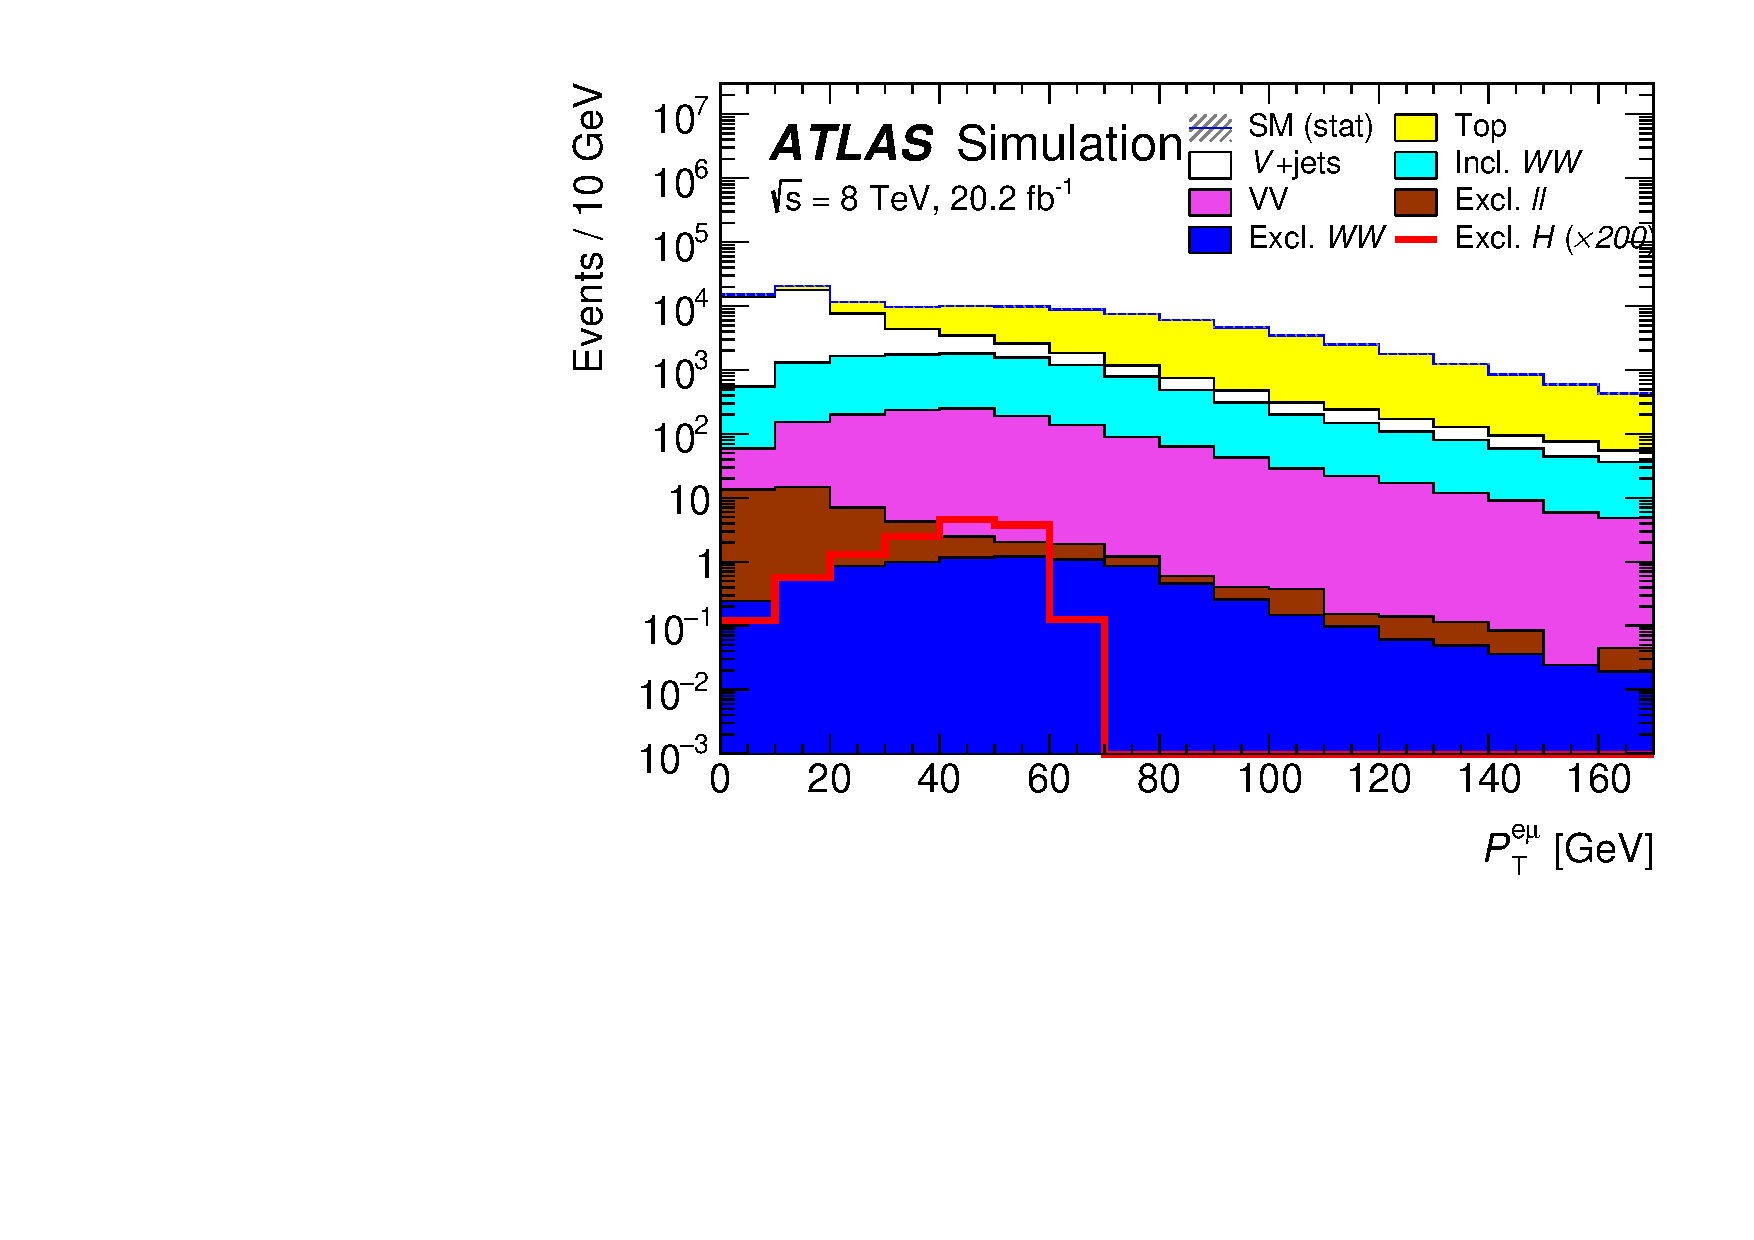
\includegraphics[width=\textwidth]{figures/emme-CutMll-Ptll-log.pdf}
\end{subfigure} 
\caption{Plots showing the expected signal and background distributions after pre-selection}
\label{fig:preselExclH}
\end{figure}

\par Figure~\ref{fig:preselExclH} shows expected distributions for several kinematic quantities for background 
and signal after the pre-selection criteria has been applied. Contributions from all the backgrounds are stacked on each 
other to total the Standard Model (SM) prediction. The hashed lines on the SM prediction is the statistical 
uncertainty, obtained by assuming that the predicted number of events follow a Poisson distribution. 
The signal prediction is not stacked on the background, and is scaled by 200 for better visibility. 
While these distributions were predicted by simulation, a full discussion on background 
treatment is detailed in Section~\ref{sec:bkgExclH}.

\par The mass of the di-lepton system, \memu, has already been introduced above. While most of the backgrounds 
have reasonably high \memu, almost all the signal is 
expected to fall in the $\memu<100~\GeV$ region, after all the pre-selection criteria has been applied. 
In particular, the $WW$ distributions tend to have high \memu\ than the signal. This is expected because with a 
spin-0 quantum number, the Higgs boson decays to final state leptons that have a smaller angular separation 
than the leptons from $WW$ decays. This small angular separation lowers \memu.   
This hints 
towards additional selection criteria dependent on the mass and angular separation of the di-lepton system.
Figure~\ref{fig:preselExclH} shows both \memu\ and \dFem, where most of the signal lies in the 
region $\dFem<2.0$.      

\par The transverse mass, \mT, of the di-lepton-\met\ system shown in Figure~\ref{fig:preselExclH} 
is defined as  

\begin{equation}
  \label{eq:mT}
  \mT = \sqrt{(E_{\mathrm T}^{e\mu}+\met)^{2} - |\boldsymbol{\pTemu} + \boldsymbol{ p_{\mathrm T}^{\mathrm{miss}}}|^{2}},
\end{equation}
where $E_{\mathrm T}^{e\mu} = \sqrt{|\boldsymbol{\pTemu}|^{2}+m_{e\mu}^{2}}$ and $|\boldsymbol{ p_{\mathrm T}^{\mathrm{miss}}}|=\met$. 
This quantity essentially is the mass of the Higgs boson, so it is expected to peak at 125~\GeV\ and have 
a small tail that is mostly in the region $\mT<140~\GeV$.

\par The transverse mass of the di-lepton system, \pTll\ or \pTemu, 
is expected to be relatively higher for signal than it is for backgrounds such as $V$+jets and 
exclusive di-leptons. QCD multi-jets, not shown in Figure~\ref{fig:preselExclH}, are also expected 
to have low \pTemu\ when the jets are mis-identified as leptons. To suppress these backgrounds, a selection 
of $\pTemu>30~\GeV$ was imposed.  

\par A dedicated selection was also developed to separate exclusive from inclusive events. This criterion 
is referred to here as the {\it exclusivity selection} or \DZ\ in short. Its perfomance in simulation and 
data was tested, and is formally introduced in the next two sections.   

\par From the distributions in Figure~\ref{fig:preselExclH} the following additional selection were applied to 
isolate Higgs-like events from the $\WW$ spectrum: $\mll<55~\GeV$, $\mT<140~\GeV$ and $\dFll<1.8$. This selection 
was found to be optimal without any additional 
 \met\ criteria.  

\par Table~\ref{tab:evSel} summarizes all the selection criteria discussed in this section. 
Figure~\ref{fig:prelimMT} shows the expected \mT\ distributions in the signal region, minus 
the \mT\ selection criterion. Modified distributions will be shown in later sections after 
several calibrations and corrections have been applied to the background processes. In any case, exclusive 
and inclusive $\WW$ was expected to dominanate the background processes that contaminated 
the signal region. 

\begin{table}
\centering
\begin{tabular}{|l|c|}
\hline
                                & Selection \\
\hline\hline
& \\
\multirow{3}{*}{Preselection } & Oppositely charged $e\mu$ final states   \\
                                				&  $\pT^{\ell 1} > 25~\GeV$ and $\pT^{\ell 2} > 15~\GeV$ \\
																		    & $\memu > 10~\GeV$     \\
& \\
\hline
& \\
				& $\pTemu > 30~\GeV$\\
                          & Exclusivity selection, \DZ\\
& \\
\hline
& \\
\multirow{3}{*}{Spin-0 Higgs boson}   & $\memu <55~\GeV$      \\
							    & $\dFem < 1.8$       \\
                                & $\mT <140$~\GeV       \\
& \\
\hline
\end{tabular}
\caption{Event selection criteria.}  
\label{tab:evSel}
\end{table}

\begin{figure}[!h]
\centering
   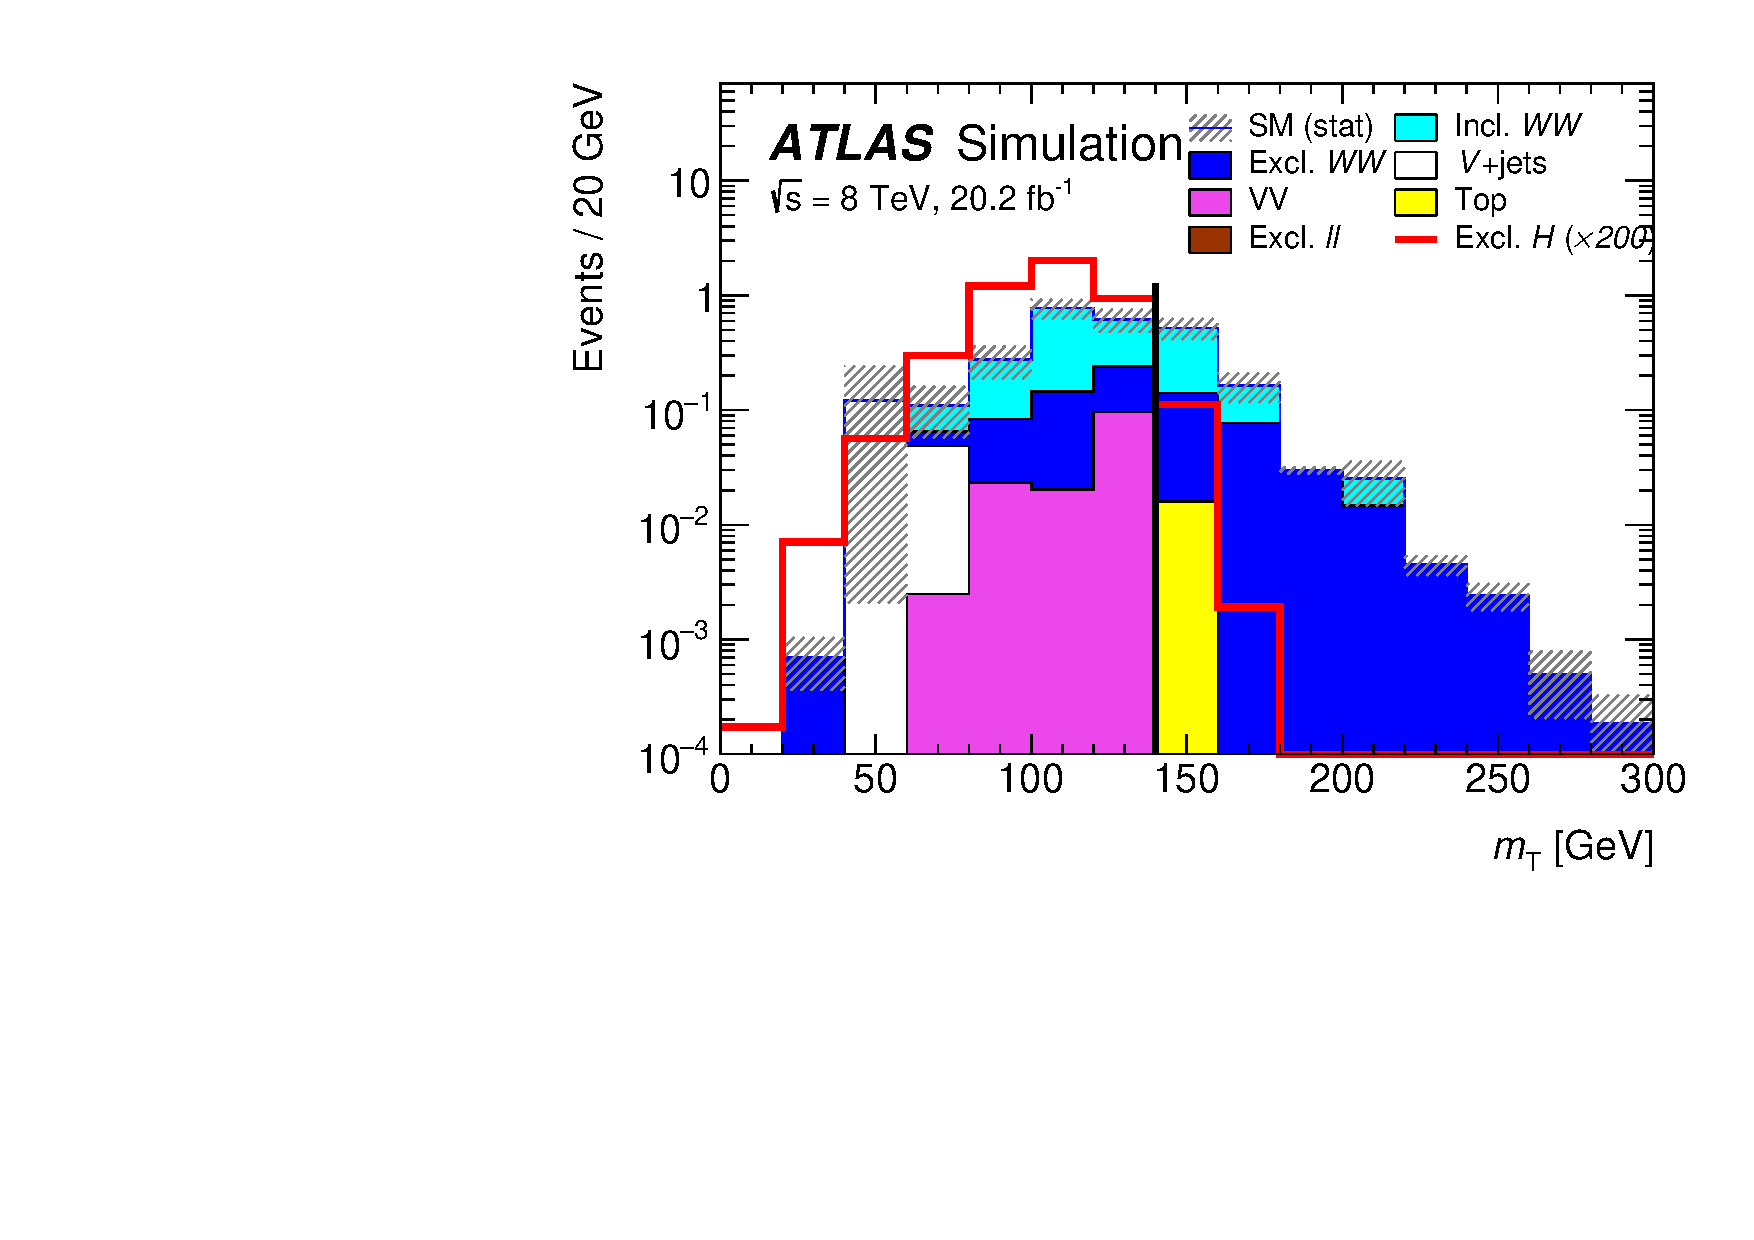
\includegraphics[width=0.8\textwidth]{figures/emme-CutDPhill-MT20-log.pdf}
\caption{Plots showing the preliminary expected \mT\ distributions in the signal region, minus the \mT\ selection}
\label{fig:prelimMT}
\end{figure}

\subsection{Exclusivity Selection}
\par The exclusivity selection developed in this analysis is based on the final state particles 
shown in the topology in Equation~\ref{eq:topExclH}. With only two leptons in the final state, these 
exclusive events are expected to have exactly two tracks in the event. These tracks are in turn expected 
to be matched to the said leptons.  

\par As mentioned in previous sections, tracks in this analysis were parametrized by impact parameters 
measured with respect to the beamline. It is worth mentioning that the most common track 
parametrization in ATLAS is with respect to the primary vertex (PV), defined as the vertex with the 
highest track sum \pt. The default ATLAS primary vertex is referred to as PV in this text, and the vertex from which two tracks 
in exclusive processes originate is referred to as the di-lepton vertex. The 
probability that a track from pileup events is mistakenly associated with the PV, especially 
in events that have few tracks, is substantial. When that happens, the position of the PV in 
the $z$ coordinate may get distorted. This, as will be shown in the next paragraphs, would reduce 
the efficiency of the exclusivity selection. So an effort to refrain from using quantities that 
rely on the ATLAS PV was made.  

\par As shown in Chapter~\ref{obj}, the fit method used to reconstruct tracks is different 
from that used to reconstruct electron tracks in the ID. In addition, the measured ID hits for 
muons candidates may be different as the combined MS+ID track fit is used for CB muons. Thus, 
matching tracks to leptons in necessary. A track was considered matched to a lepton track if it 
satisfied the following conditions :
\begin{enumerate}
\item passes all track quality selection criteria;
\item has at least 2~\GeV\ in \pt;
\item $\Delta z_0(\text{track,lepton})$ is less than 1 mm;
\item and $\Delta R(\text{track,lepton})$ is less than 0.01.
\end{enumerate}   
In the case where a track is matched to both leptons in the event, preference is given to the lepton 
closest in $z_0$, measured with respect to the beamline. Figure~\ref{fig:trkMatch} shows the number of tracks 
matched to electrons and muons in the  simulated signal sample of events. Electrons, since they undergo 
brehmsstrahlung at a higher rate than muons, have a larger fraction of two matched tracks than muons. It 
is not expected to match 3 or more tracks to either of the leptons. 

\begin{figure}[!h]
\begin{subfigure}{0.5\textwidth}
   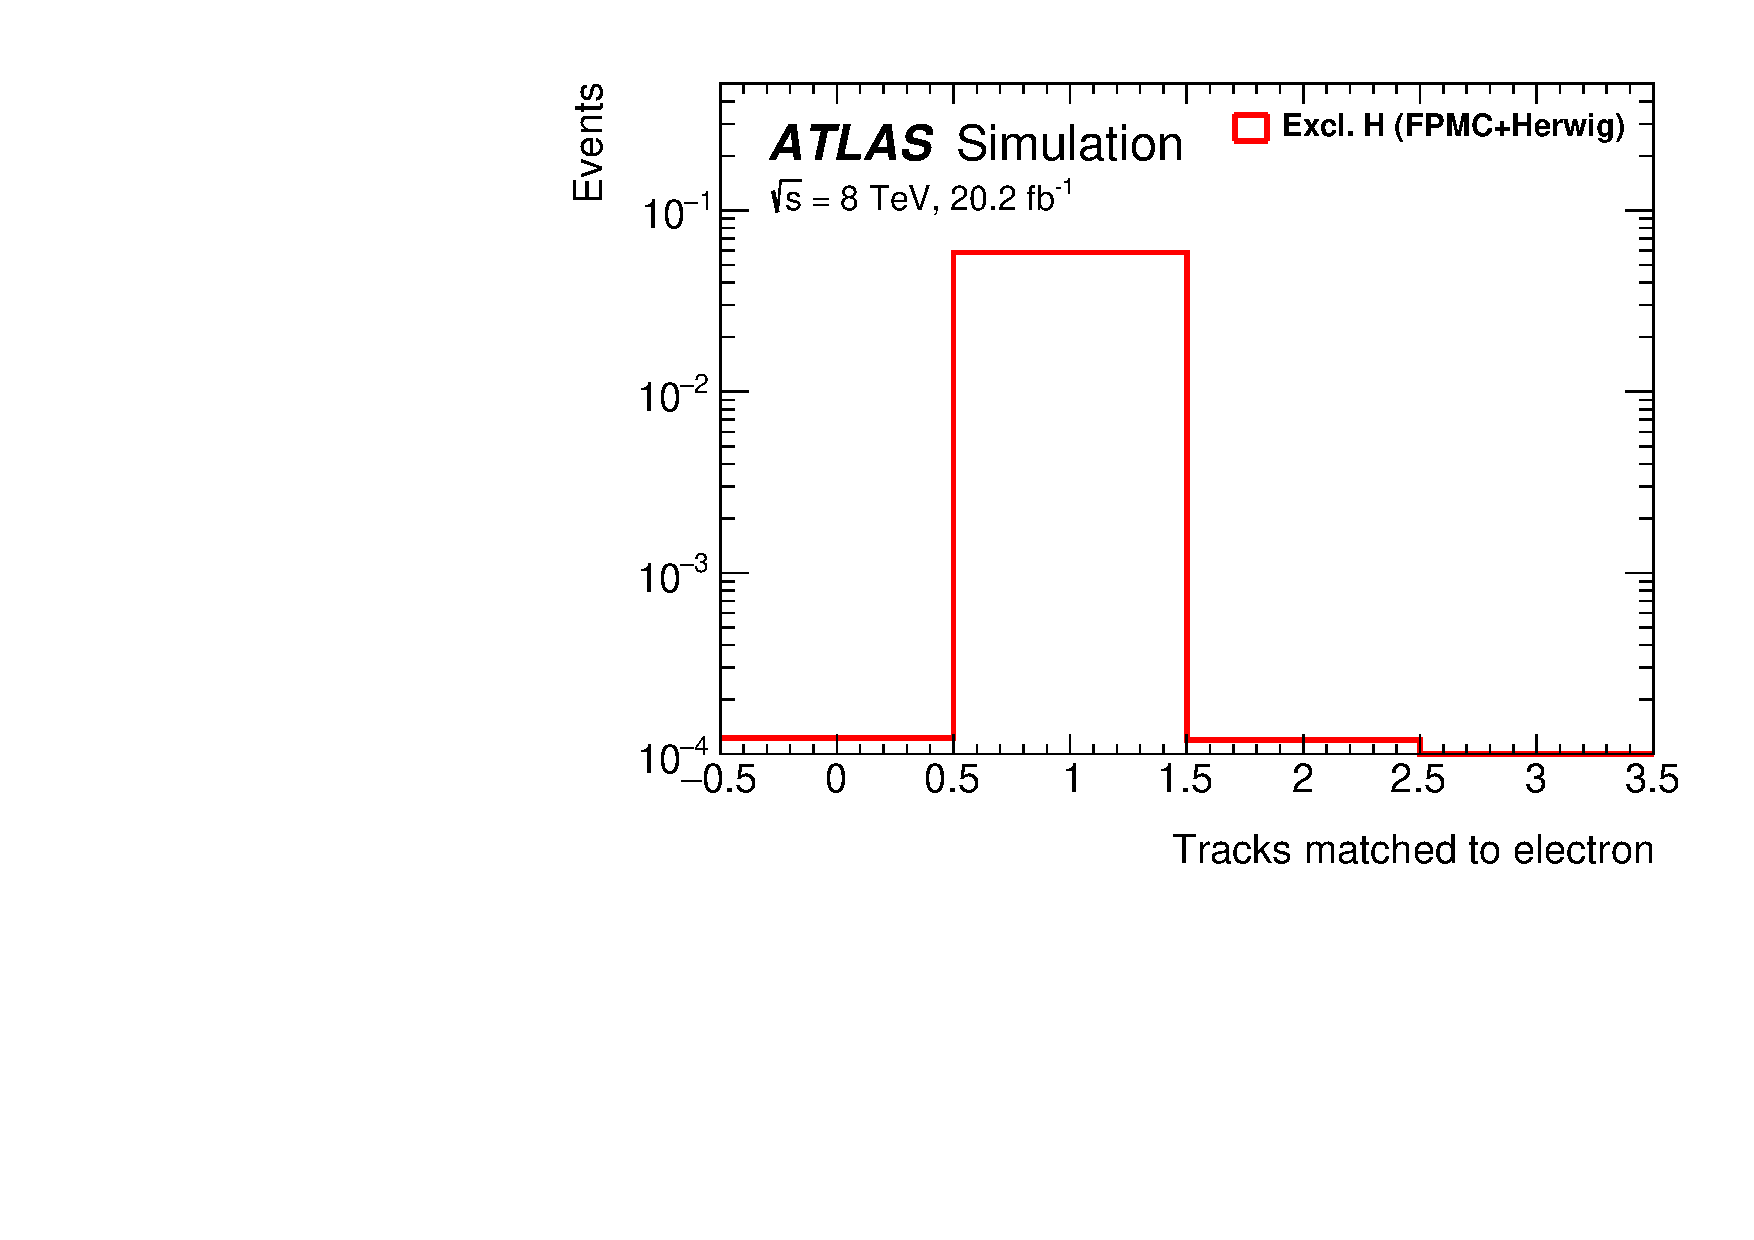
\includegraphics[width=\textwidth]{figures/em-CutChannels-nTrkMatch0-log.pdf}
\end{subfigure}%
\begin{subfigure}{0.5\textwidth}
   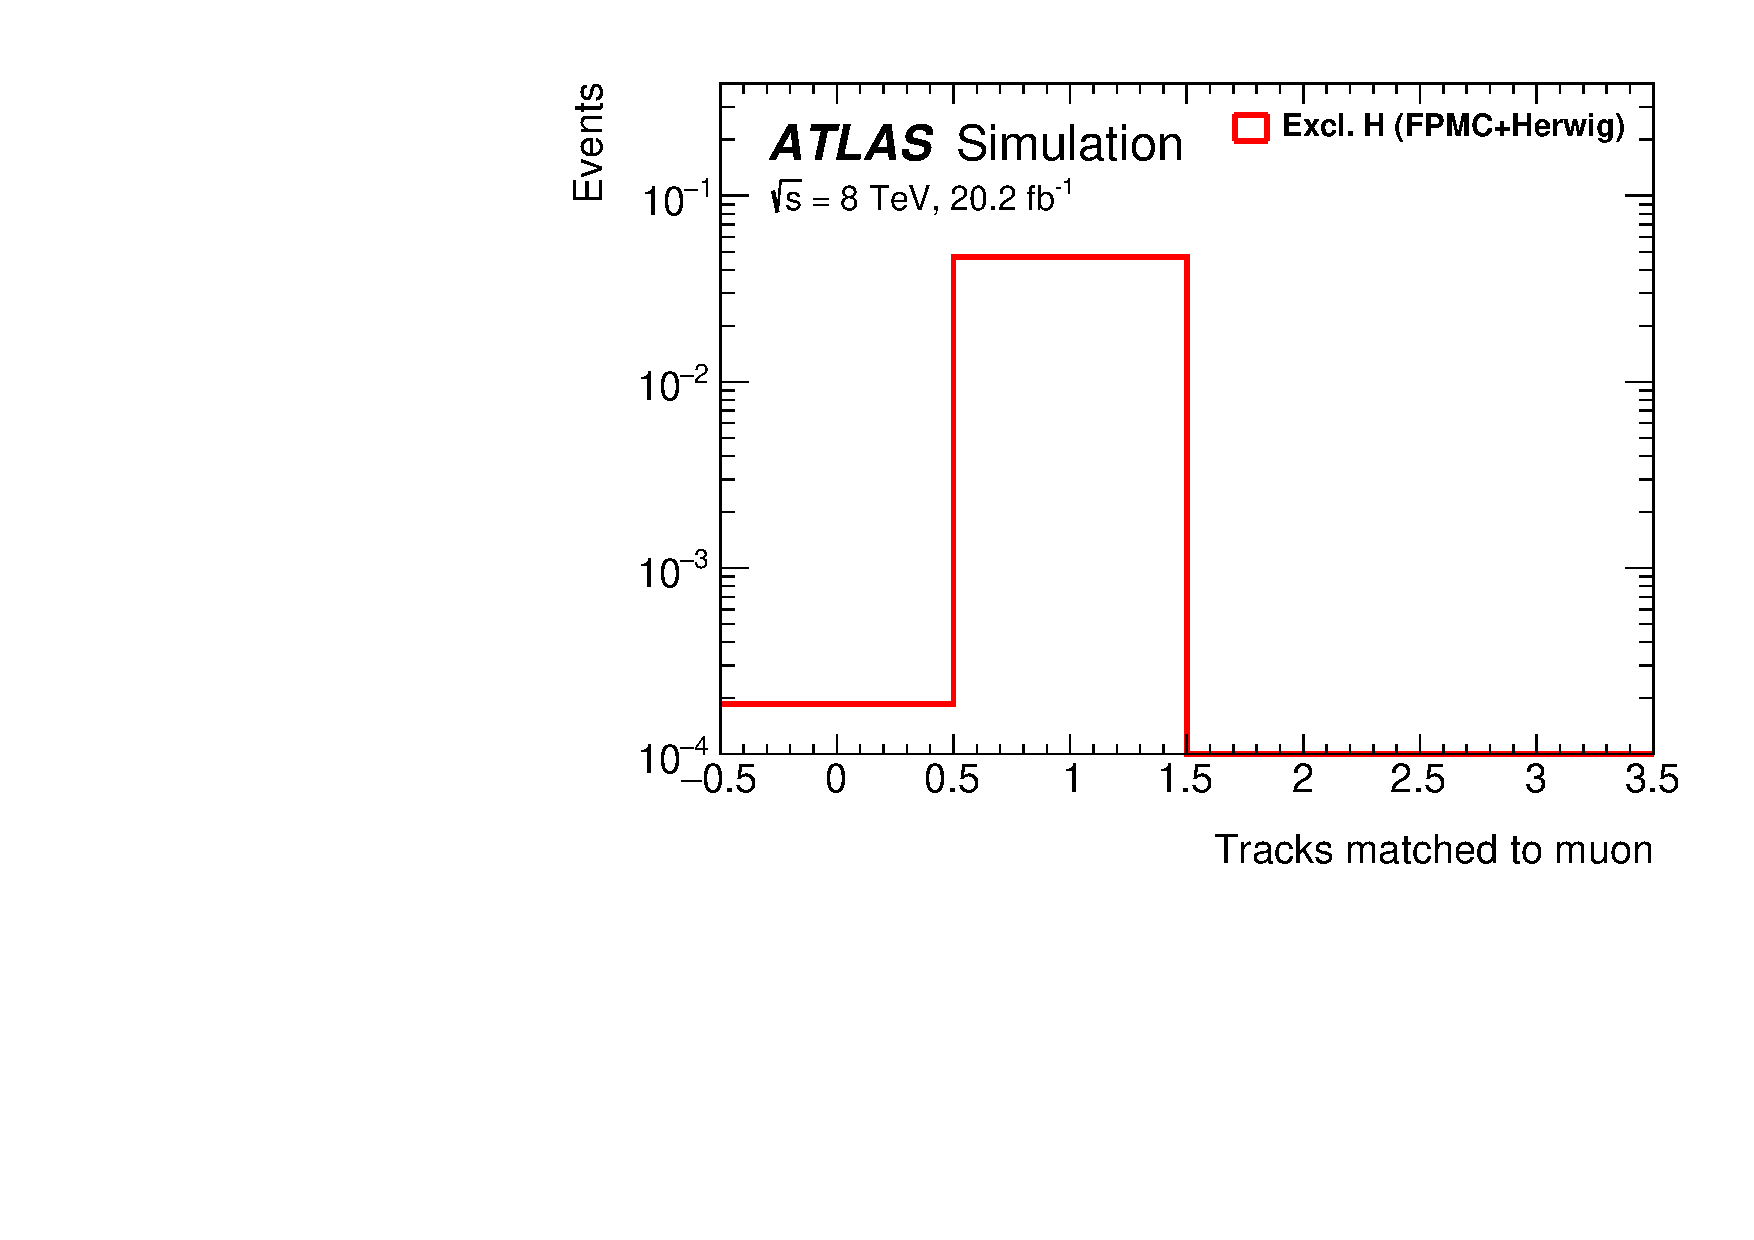
\includegraphics[width=\textwidth]{figures/me-CutChannels-nTrkMatch0-log.pdf}
\end{subfigure} 
\caption{Plots showing the number of tracks matched to the electron (left) and the muon (right) tracks}
\label{fig:trkMatch}
\end{figure}

\par To ensure that the two leptons in the event are indeed from the di-lepton 
vertex, their $z_0$ positions, $z_0^1$ and $z_0^2$, were required to be within 1 mm of each other. 
The 1 mm value was arrived at after measuring the $z_0$ resolution in both data and simulation and 
observing that they safely agree within 1 mm. The position of the di-lepton vertex in $z_0$, $z^{av}_0$, was then 
taken as the average of $z_0^1$ and $z_0^2$. Tracks not matched to either of the leptons 
were tested for absolute distance in $z_0$ from $z_0^{av}$. Figure~\ref{fig:exclCartoon} 
illustrates this geometry. For \DZ, the closest unmatched track (also referred to as an {\it extra} track) 
was required to be at least 1 mm way from $z_0^{av}$. 

\begin{figure}[!h]
\centering
   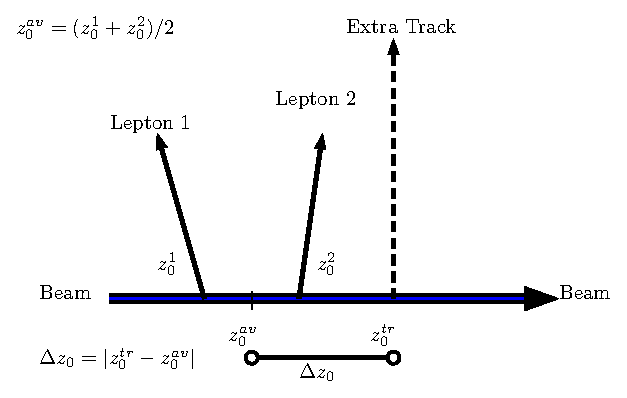
\includegraphics[width=0.8\textwidth]{figures/cartoon.eps}
\caption{Illustration of the geometry of the exclusivity selection criteria}
\label{fig:exclCartoon}
\end{figure}

\par Although \DZ\ was observed to be sensitive to pileup events, the signal selection 
efficiency in the pileup range expected during the Run I data taking period was not terrible. At 
worst the signal efficiency was about 50\%, when the number of pileup events ($\mu$) was 
greater than 30. During Run I, the average number of pileup events was 20.7. Figure~\ref{fig:pileupEff} 
shows the signal efficiency of this selection, simulated using FPMC, plotted against 
the number of pileup event, $\mu$. For $\mu=20.7$, the efficiency was found to be around 58\% 
in simulation. The was compared to the efficiency measured in data, as discussed in the 
next section. 

\begin{figure}[!h]
\centering
 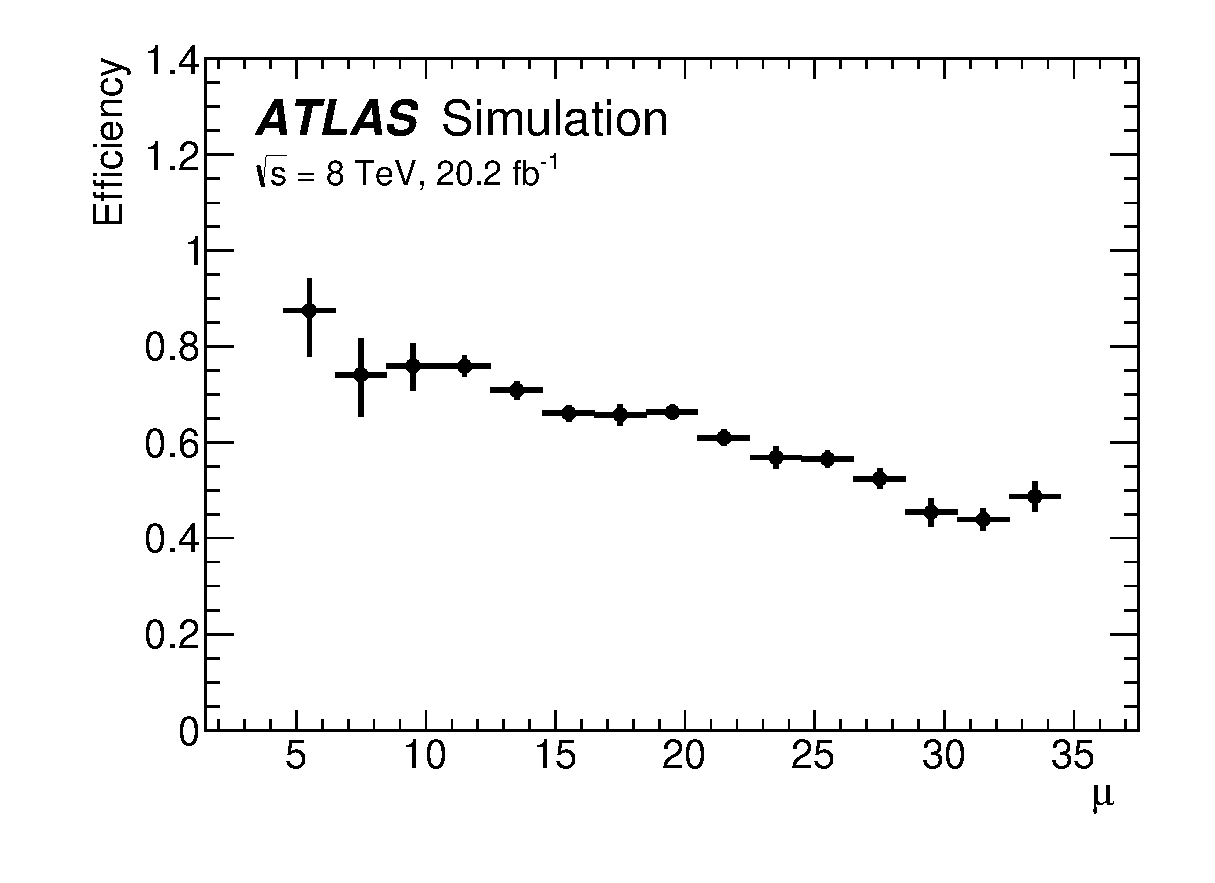
\includegraphics[width=0.8\linewidth]{figures/muFit.eps} 
\caption{Plot of the efficiency of the exclusivity selection, extracted from the
exclusive Higgs boson signal simulation, is plotted 
against the average number of interactions per beam crossing
$\mu$}
\label{fig:pileupEff}
\end{figure}

\subsection{Performance and calibration of exclusivity}
\label{sec:exclCalib}
\par The exclusivity selection introduced in the previous section was tested for several 
inconsistencies in data and simulation. First, since background rejection with this selection in 
simulation is dependent on the modelling of the underlying event, it is reasonable to 
expect difference in performance in different Monte Carlo generators as well as in data. 
Second, the equivalent photon approximation (EPA) is known to overestimate the cross section of 
elastic processes such as elastic di-leptons or elastic \Wpm\ pairs~\cite{Dyndal,Harland-Lang:2015cta}.
It was worthwhile to reproduce this over-estimation using \DZ\ as a cross check.  
Third, SD and DD Monte Carlo simulation for exclusive \Wpm\ pairs is not available. A mechanism to estimate 
these contributions was developed in the context of \DZ. 

\par This section discusses three studies. The underlying event modelling in several 
Monte Carlo generators were calibrated to match the underlying event in data. The EPA 
overestimation of elastic cross sections were reproduced using the \DZ\ selection criteria. 
SD and DD contributions to the exclusive \Wpm\ pairs was estimated. These three studies 
essentially tested the perfomance of \DZ\ and enabled its calibration.  

\subsubsection{Calibration of the underlying event}
\par To calibrate the underlying event modelling across different generators, \Zmm\ events in data 
were used for comparison. \Zee\ samples were also used separately to cross check the results. The reason for 
using Z events is that while they are a good source of leptons, they are so many in data that 
statistical uncertainties are kept at a minimum. The Z events were isolated by requiring each of the two muons 
to have at least 20~\GeV\ in \pt\ and have $80<m_{\mu\mu}<100~\GeV$. \DZ\ was then applied, essentially 
requiring no unmatched tracks in $\pm\Delta z_0<1$ mm. The $\pm\Delta z_0$ window was varied to study 
systematic uncertainties on the results. 

\par The following generators were used to simulate \Zmm\ events :
\begin{enumerate}
\item \AlpgenPythiaSix; 
\item \AlpgenHerwig;
\item \SHERPA;
\item and \POWHEG+\PYTHIAeight.
\end{enumerate} 
Figure~\ref{fig:zsubcut} shows the agreement between data and simulations from these generators. 
Circles and squares are respectively before and after the exclusivity selection was applied. Before 
exclusivity, all the generators predict \Zmm\ events to a reasonable agreement with data. After 
exclusivity, several disagreements between data and simulation, and also between simulations from the 
different generators, were observed. This is a symptom of poor underlying event modelling.  

\begin{figure}[!h]
\centering
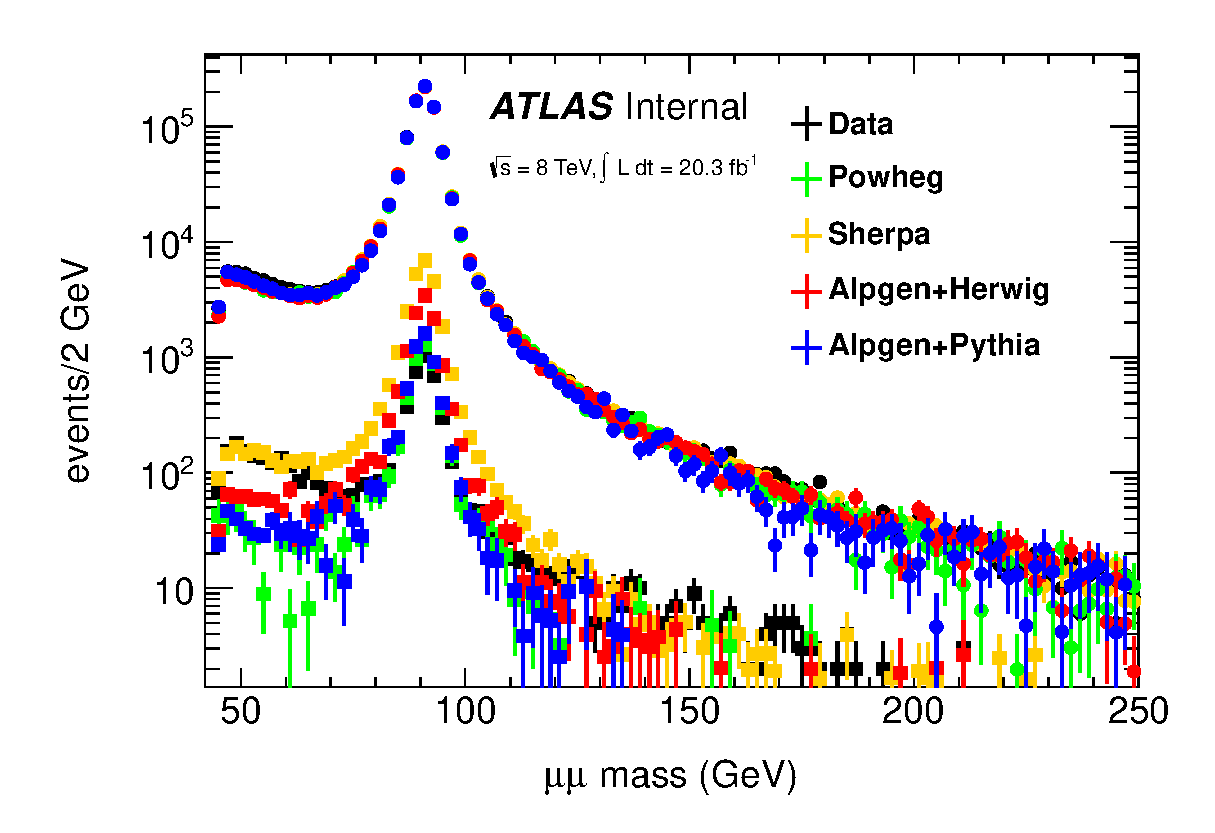
\includegraphics[width=0.8\linewidth]{figures/zrejcal.eps}
\caption{The rejection of \Zmm\ between data and simulation. Simulated samples are normalized to the
data. Circles are before \DZ\ was applied, and squares are after \DZ\ was applied}
\label{fig:zsubcut}
\end{figure}

\par The fraction of events that passed \DZ\ in simulation, $n^{exc}_{MC}/n^{inc}_{MC}$, and the fraction of events 
that passed \DZ\ in data, $n^{exc}_{data}/n^{inc}_{data}$, were compared through scale factors   

\begin{equation}
f^{sim}_{n_{trk}} = \frac{n^{exc}_{MC}/n^{inc}_{MC}}{n^{exc}_{data}/n^{inc}_{data}}, 
\label{eqn:rsf}
\end{equation}
where {\it sim} is $P$ for \POWHEG+\PYTHIAeight, $AH$ for \AlpgenHerwig, AP for \AlpgenPythiaSix,
and $S$ for \SHERPA. $n_{trk}$ is the number of tracks required in the exclusivity window, 0 
being the nominal. To improve the statistical uncertainties after \DZ, measurements with $n_{trk}$ equal 
to 1 and 1$\to$4 were also done. Exclusivity window sizes other than 1 mm were used to study 
the impact of systematic uncertainties on the results. Results for this study are shown in 
Table~\ref{tbl:rejscale}.  

\begin{table}[h]
\begin{center}
\begin{tabular}{|l|cccc|}
\hline
$n_{trk},  \Delta z^{iso}_0$ & $f^P_n$ & $f^S_n$ & $f^{AH}_n$ & $f^{AP}_n$ \\
\hline\hline
0, 1.0 mm & 0.581 & 0.128 & 0.206 & 0.692 \\
0, 1.25 mm & 0.549 & 0.113 & 0.194 & 0.679 \\
0, 1.5 mm & 0.537 & 0.103 & 0.189 & 0.663 \\
0, 2.5 mm & 0.494 & 0.084 & 0.176 & 0.613 \\
0, 4.0 mm & 0.308 & 0.074 & 0.170 & 0.579\\
1-4, 1.0 mm & 0.876 & 0.571 & 0.393 & 0.853 \\
1, 1.5 mm & 0.681 & 0.324 & 0.247 & 0.736 \\
\hline
\end{tabular}
\caption{Measured $f^{sim}_{n_{trk}}$ values for several different Monte Carlo generators, under different exclusivity 
settings. Exclusivity window sizes other than 1 mm were used to study the impact of systematic variations on the results.} 
\label{tbl:rejscale}
\end{center}
\end{table}

\par To use the scale factors in Table~\ref{tbl:rejscale} to calibrate processes other than $Z$ decays 
these scale factors were extrapolated to a wider di-muon mass range. In particular, the stability of event
yields after imposing \DZ\ at di-muon masses other than between 80 and 100~\GeV needed to be quantified. These simulation yields 
 were measured in bins of $44\to60~\GeV$, $60\to90~\GeV$, $90\to116~\GeV$ and $116\to200~\GeV$. In all bins, \SHERPA had the 
minimal statistical uncertainties, so its results were compared to those from the other three generators. Quantities 
shown in Table~\ref{tab:gencm} are ratios of yields from the different generators to the yields from \SHERPA after 
the \DZ\ selection. A generous 20\% variation on the nominal yield (\SHERPA) covers yields from all other 
generators.  

\begin{table}
\begin{center}                                                                 
\begin{tabular}{l|c|c|c}                                                       
\hline                                                    
Mass [\GeV]  & \AlpgenHerwig & \AlpgenPythiaSix  & \PowhegPythiaEight  \\    
\hline         
 44--60  & $0.81 \pm 0.02$  & $0.84 \pm 0.03$ & $0.99 \pm 0.09$\\     
 60--90 & $1.04 \pm 0.02$  & $0.98 \pm 0.03$  & $1.01 \pm 0.02$\\     
 90--116 & $1.00 \pm 0.01$ & $1.02 \pm 0.02$  & $1.00 \pm 0.02$ \\  
 116--200 & $0.89 \pm 0.10$& $1.04 \pm 0.19$  & $0.76 \pm 0.10$\\    
\hline      
\end{tabular}                     
\caption{Ratio of the exclusivity selection efficiency in Drell-Yan
 $\mu^+\mu^-$
production as a function of dimuon mass of different generators to
\SHERPA. Only statistical uncertainties 
are shown. The statistical uncertainty from \SHERPA is included and contributes $2.9\%, 0.8\%,
0.7\%$ and $5.7\%$ in the four mass regions.}
\label{tab:gencm}            
\end{center}             
\end{table}

%\par Talk about validation of scale factors ... show Figure 7 from the paper ...


\subsubsection{Di-lepton check}
\label{sec:acofit}
\par As mentioned above, the EPA is known to overestimate the elastic contribution to exclusive processes 
that occur by exchanging a pair of photons. This section discusses a study that reproduces this overestimation 
within uncertainties, thereby validating \DZ. 

\par Since elastic, SD and DD Monte Carlo simulation samples for exclusive di-leptons were available, exclusive 
di-leptons were used for this study. The strategy was to isolate exclusive di-muons in data, entangle the 
elastic component, and compare it with the prediction from EPA. From this comparison, a scale factor than normalizes 
the EPA prediction to data was extracted and compared to previous studies of a similar nature. The basic selection required 
that each of the muons have $\pt>20~\GeV$, $m_{\mu\mu}>45~\GeV$ excluding a $\pm15~\GeV$ window around the 
\Zboson\ mass, and \DZ. Elastic di-muons tend to populate the low \pTmumu\ region, as shown in 
Figure~\ref{fig:ptL}, where all the basic selection criteria described above were applied. 
So, a selection of $\pTmumu<3~\GeV$ was additionally applied.  
The major background 
to the exclusive di-muons in this region was Drell-Yan di-muons; every other background was negligible.  
Clearly, in Figure~\ref{fig:ptL} there is an overestimation of processes from simulation. 

\begin{figure}
\centering
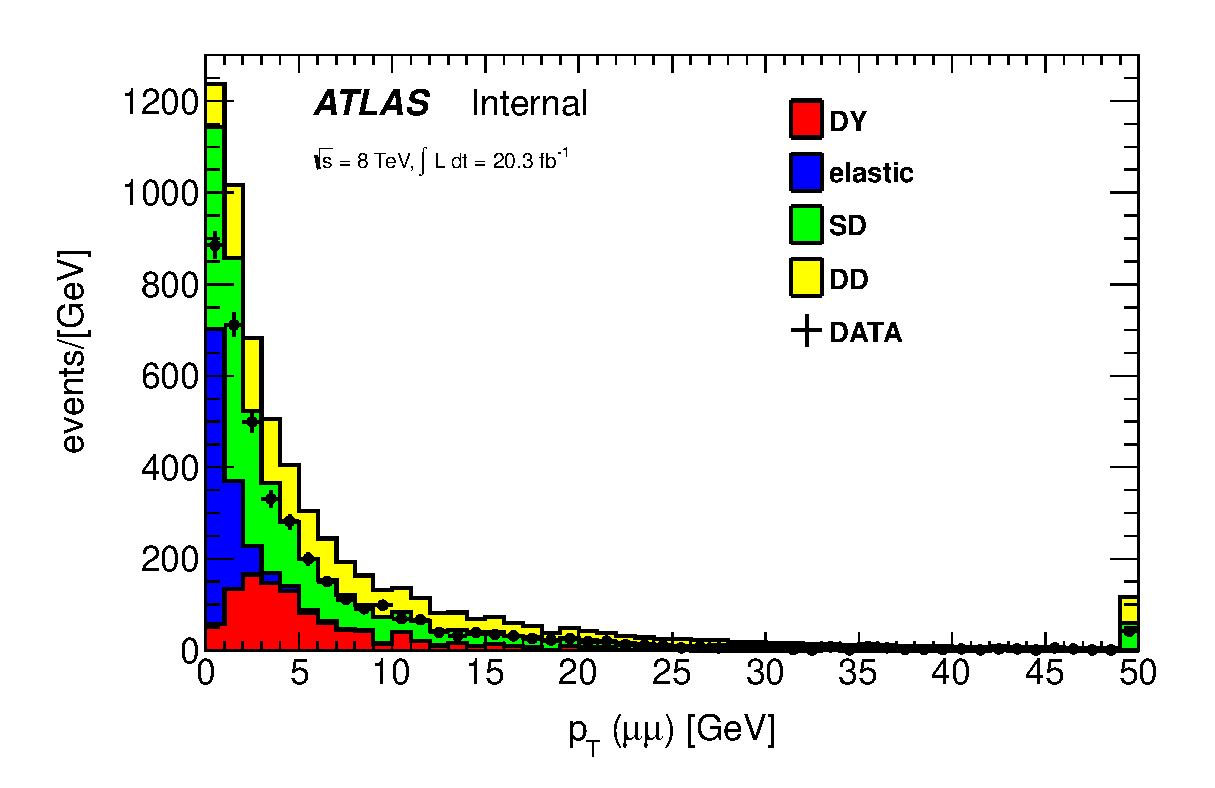
\includegraphics[width=0.8\linewidth]{figures/ptmumuL.eps}
\caption{Plots showing the exclusive (1.0 mm) di-muon $p_{\mathrm{T}}^{\mu\mu}$ distributions predicted and observed. The
  highest bin includes overflow. No scale factors are applied to
  elastic or SD or DD predictions}
\label{fig:ptL}
\end{figure}

\par Acoplanarity, defined as $1-\Delta\phi_{\mu\mu}/\pi$, is a good discriminant when disentangling elastic 
from SD and DD processes. This is expected, since $\Delta\phi_{\mu\mu}$ is dependent on \pTmumu. In this study, 
acoplanarity distributions from simulation after applying the selection criteria described in the preceding paragraphs   
were fit to the acoplanarity distribution from data, after the same selection criteria was applied. 
The yields from the fit were then extracted, comparing the elastic prediction to data minus everything else. 

\par The acoplanarity distributions before the fit are shown in Figure~\ref{fig:shapes}. Clearly, SD, DD and 
Drell-Yan have similar shapes. For the fit, SD, DD and Drell-Yan contributions were summed up and treated as 
one process. The Drell-Yan background was varied by $\pm20\%$ to evaluate systematic variations in modelling 
$f^{sim}_{n_{trk}}$. The binning and range of acoplanarity distributions were also varied to evaluate 
systematic uncertainties. These uncertainties were shown to impact results by about 7\%. 
Figure~\ref{fig:dilepAcoFit3Shape} shows the post-fit acoplanarity distributions, with 
simulation stacked on top of each other and the total agreeing with the data. From this fit a scale factor 
 $f_{EL}$ = 0.76 $\pm0.04$ (stat.) $\pm0.07$ (sys.) was extracted. This value agrees within uncertainties with 
previous predictions~\cite{Dyndal}, which cover a range between 0.73 and 0.75.   

\begin{figure}[!h]                                                                 
\centering
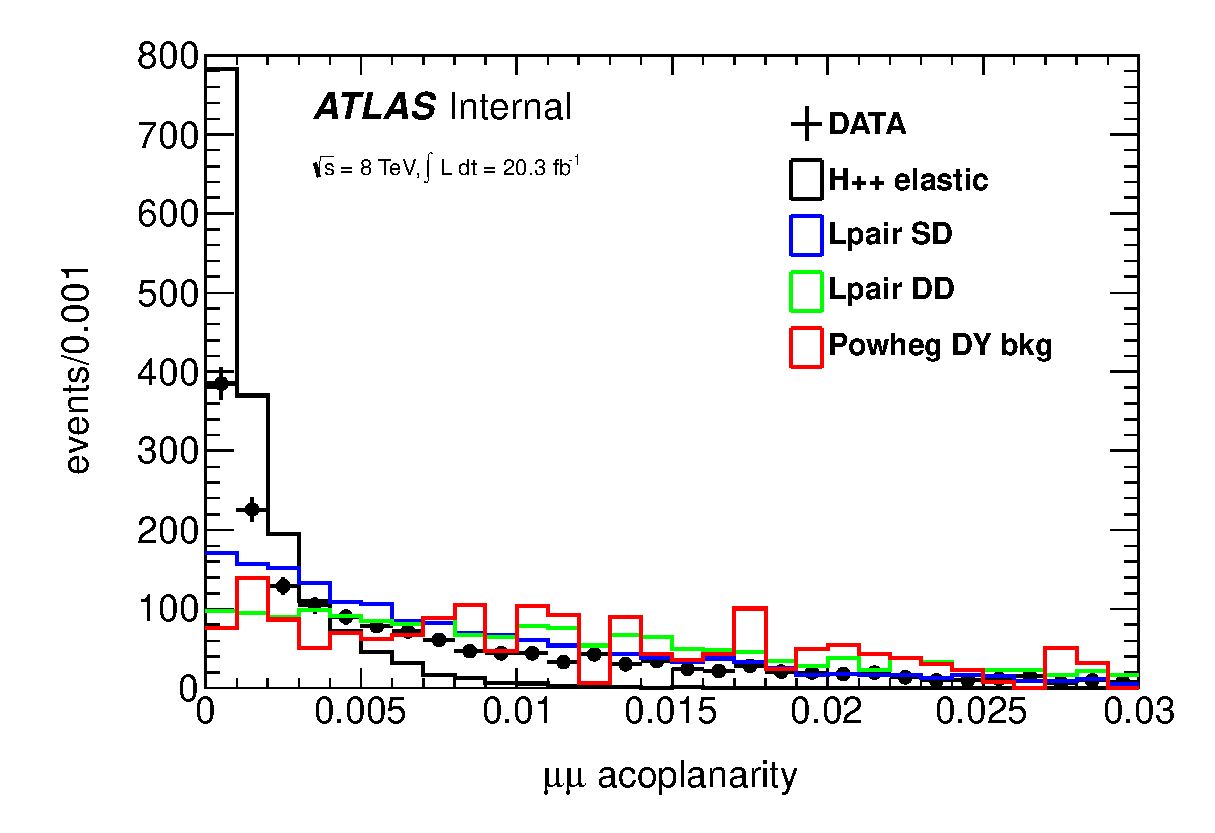
\includegraphics[width=0.8\linewidth]{figures/shapes.eps}     
\caption{Plots of acoplanarity distributions for elastic, SD, DD and Drell-Yan
each normalized to the data}                                             
\label{fig:shapes}                        
\end{figure} % 

\begin{figure}[!h]                                                                 
\centering
 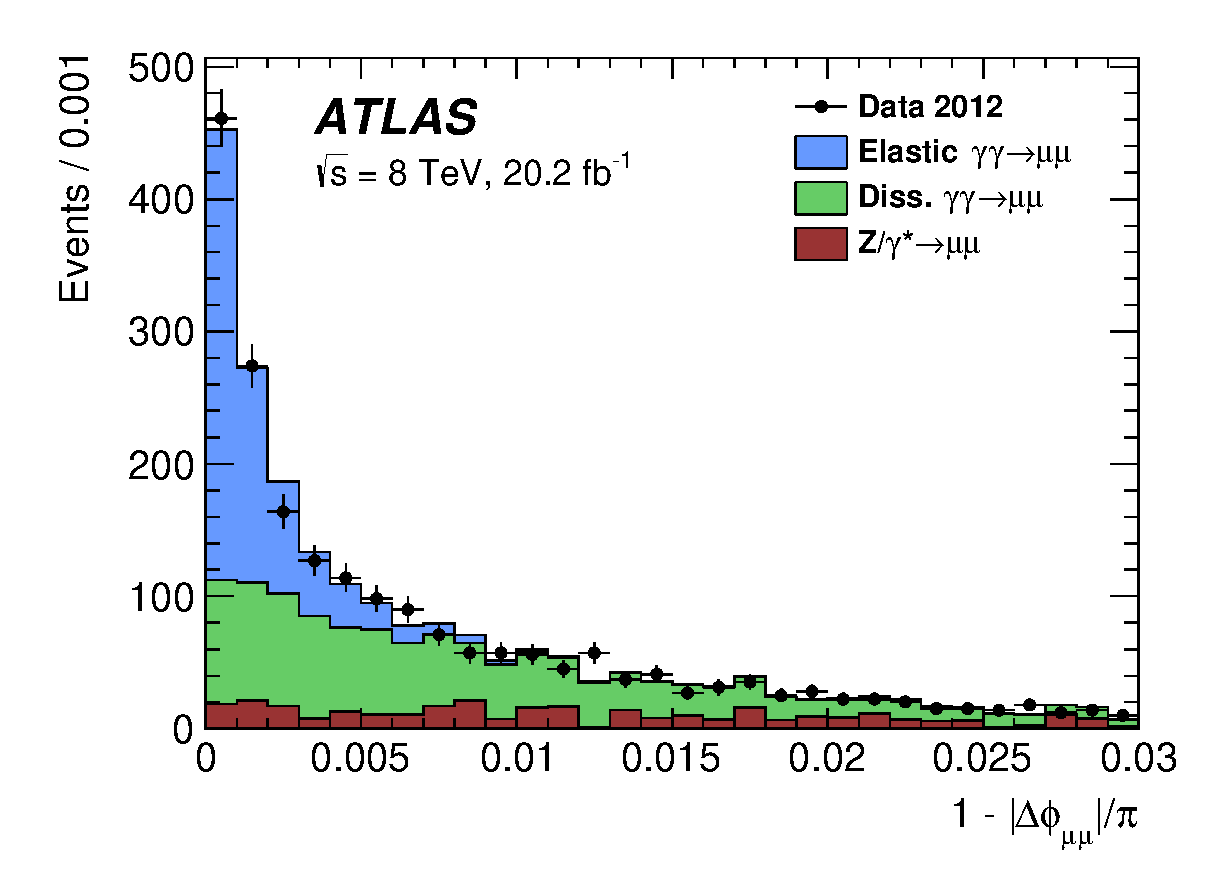
\includegraphics[width=0.8\linewidth]{figures/dilepton_3shapes_Washington_filled.eps} 
 \caption{Plots of dimuon acoplanarity distributions after applying the
 exclusivity selection and requiring $\pT^{\mu\mu} < 3$~\GeV. The 
 expected Drell-Yan shape and the 
 elastic and combined SD and DD (Dissociative) shapes normalized from
 the fit are stacked. This fit 
          determines the factor $\fEL$.}
 \label{fig:dilepAcoFit3Shape}
\end{figure}                                        

\par A separate study independent of the fit method was also done to test the robustness of \fEL. 
This involved making an explicit selection based on acoplanarity in addition to the basic requirements 
already discussed above, counting the yields and re-calculating an estimate to \fEL. For acoplanarity less than 0.003, 
899 events were observed in data, 764 elastic dimuons were predicted by EPA, and 340, 67 and 64 SD, DD and Drell-Yan 
events were also predicted respectively. This corresponds to an estimate to \fEL\ of 
 $0.71 \pm0.03 \text{(stat)} \pm0.01 \text{(sys)}$. 
Similarly, tightening the acoplanarity selection to be less than 0.0015 yielded 0.73 $\pm0.03 \text{(stat)} \pm0.01 \text{(sys)}$.
These results fall well within the uncertainties of the results obtained from the fit method. 

\par \DZ\ was tested for robustness against pileup by testing its performance in events with a selection identical to 
the one prior to the fit plus an acoplanarity cut, with the difference that one extra track was allowed in the exclusivity 
window. For exclusive processes, this extra track has to be from pileup because there is no underlying 
event. As such, the $\Delta z_0$ between this extra track and the di-lepton vertex is expected to be 
uniformly distributed, showing no clear peaks. Figure~\ref{fig:dzEventOneTrk} shows the  $\Delta z_0$ 
distributions for the extra track in exclusive and \Zmm\ events. For exclusive processes these 
distributions are uniform while for \Zmm\ a they peak at 0. This shows that for \Zmm\ the extra track 
is from the underlying event. The acoplanarity cut was tightened and loosened and an estimate of \fEL\ was 
computed at each variation. All the \fEL\ estimates fell within $\pm10\%$, showing that \DZ\ has an a 10\% 
pileup uncertainty.   

\begin{figure}[!h]
\centering
 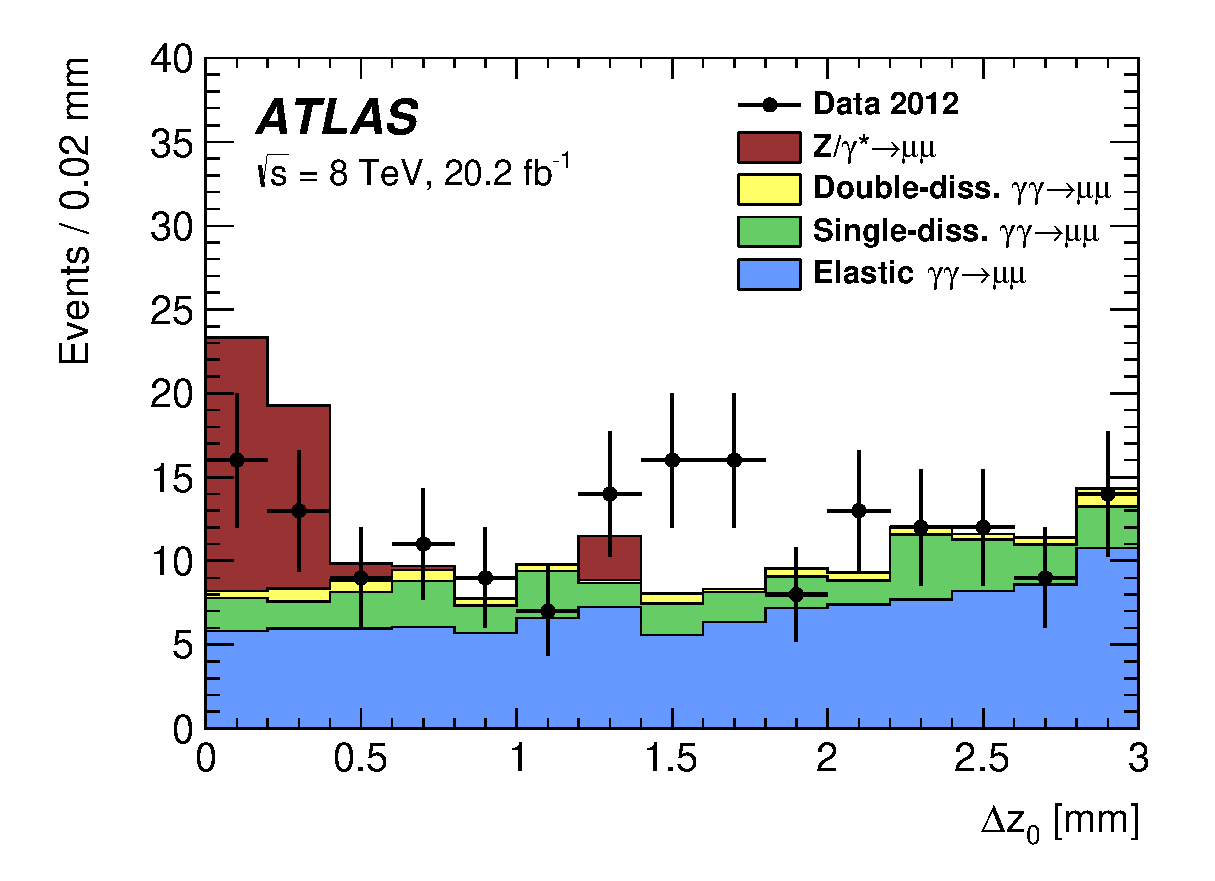
\includegraphics[width=0.8\linewidth]{figures/dilepton_dzone15.eps} 
 \caption{Plots of absolute $\Delta z_0$ of the extra track to the lepton vertex 
          in the region defined by acoplanarity $<0.0015$. The exclusivity 
          requirement was changed to select exactly one
          extra track within 3~mm.  The exclusive predictions are
 scaled by a factor of 0.70}
 \label{fig:dzEventOneTrk}
\end{figure}

\par Since electrons are also in the signal final state, these studies were repeated using 
\Zee\ events. Due to the fact that electrons undergo brehmsstrahlung at a much higher rate than 
muons, results in the \Zee\ channel carried a much higher error. In particular, when an electron 
radiates a photon (which pair produces electrons), the extra track that the radiated electron produces 
in the ID may be counted as an extra track by \DZ. This phenomenon is referred to here as 
{\it electron self-veto}. For acoplanarity less than 0.003 the estimate to \fEL\ obtained 
through \Zee\ events was about 0.67. For acoplanarity less than 0.0015 it was 0.68. These results 
correspond to a $3.0\pm 2.5\%$ difference with the results obtained from \Zmm. This difference was 
taken as the uncertainty due to the electron self-vetoing itself.   

\subsubsection{Photon flux}
\label{sec:flux}
\par This section discusses the estimation of SD and DD \Wpm\ contributions to the exclusive 
\Wpm\ pair production. This is an important estimation because it propagates to the estimation of 
the exclusive \Wpm\ pair contamination in the exclusive Higgs boson signal region.  

\par Since exclusive di-lepton production is identical to exclusive $\WW$ production, 
this study was conducted with exclusive di-leptons. The results were then 
applied to exclusive $\WW$. The strategy was to isolate exclusive di-leptons with high mass  
in data and taking the ratio of the data minus background to the elastic di-lepton prediction. 
This ratio was then applied to the elastic $\WW$ prediction to account for the SD and DD contributions. 
As before the leptons used were di-muons, each of at least 20~\GeV\ in \pt. To suppress di-muons from 
$\WW$ decays, $m_{\mu\mu}$ was required to be at least 160~\GeV. After applying \DZ, 244 events were 
observed in data were 17.4 was predicted to be from Drell-Yan, 0.4 from inclusive $\WW$ and 2.4 from exclusive 
$\WW$. The predictions were corrected using the $f^{sim}_{n_{trk}}$ calibrations. From these quantities a scale factor 

\begin{equation}
 \fgam = \frac{N_{\mathrm{Data}} 
              - N^{\POWHEG}_{\mathrm{Background}}}{N^{\HERWIGPP}_{\mathrm{Elastic}}} \Bigg\rvert_{m_{\mu\mu} > 160~\GeV}
            = 3.30 \pm 0.22 \mathrm{(stat.)} \pm 0.06 \mathrm{(sys.)},
 \label{eqn:fgamma}
\end{equation}
was calculated, where $N_{\mathrm{Data}}$ is the number of events in data, 
$N_{\mathrm{Background}}^{\POWHEG}$ is the expected number of
background events, 
and $N_{\mathrm{Elastic}}^{\HERWIGPP}$ is the expected number of elastic $\yymumu$ candidates
directly from \HERWIGPP, i.e, the unscaled EPA prediction. 
Drell-Yan processes were the major contribution to the total background events and inclusive 
and exclusive $\WW$ contributed less than 10\%. To estimate the systematic uncertainties, the Drell-Yan 
contribution was varied by $\pm20\%$. Figure~\ref{fig:fluxM160} shows the $m_{\mu\mu}$ and 
$m_{ee}$ distributions for the exclusive di-leptons after applying \fEL\ to the elastic contribution 
and scaling the SD distribution such that the sum of the elastic and SD contributions corresponds 
to $\fgam \times N_{\mathrm{Elastic}}^{\HERWIGPP}$. These corrected predictions agree very well with the data. 

\begin{figure}
 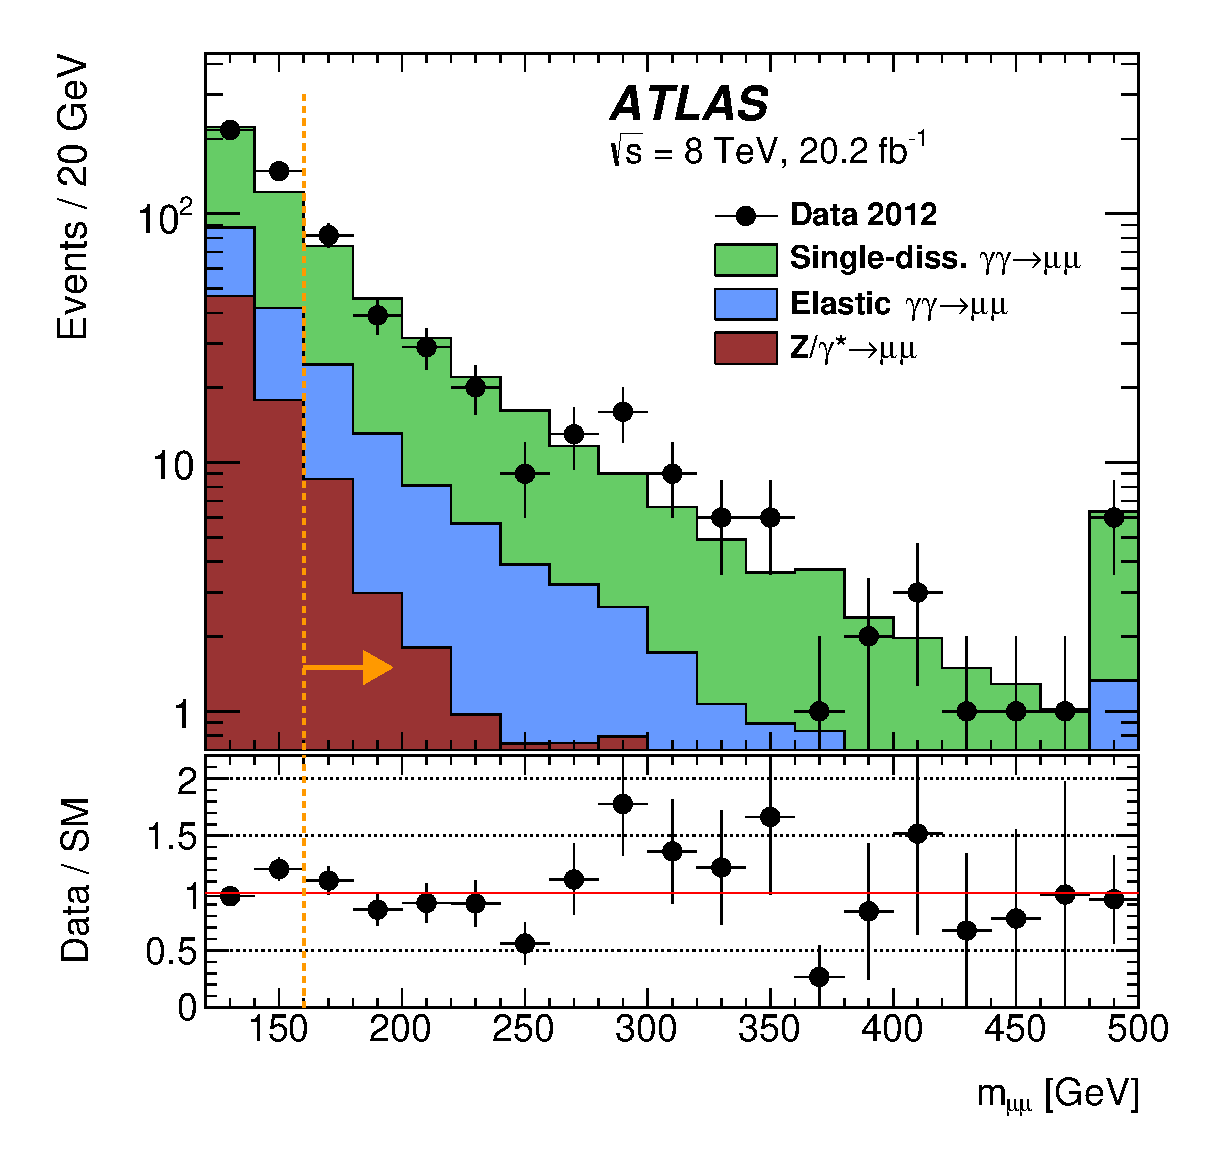
\includegraphics[width=0.5\linewidth]{figures/flux_m160mumu.eps} 
 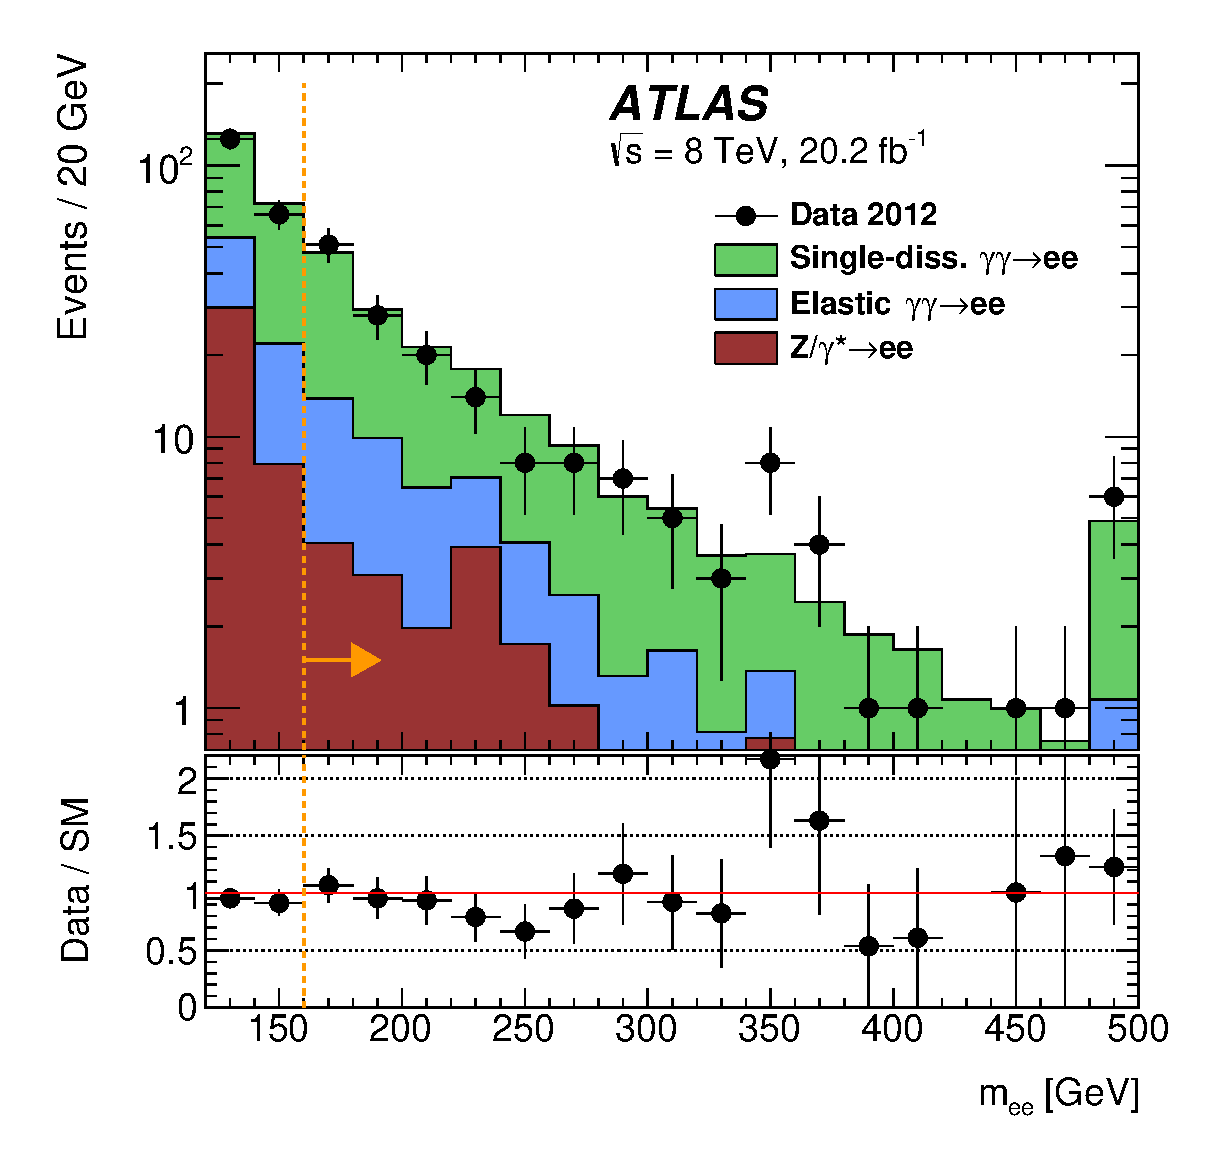
\includegraphics[width=0.5\linewidth]{figures/flux_m160ee.eps} 
 \caption{Plots of the dilepton invariant mass distribution for muon
 candidates (left) and 
          electron candidates (right). The elastic yield is scaled 
          by $\fEL = 0.76$ and the SD distribution is scaled to
          bring the sum of the elastic and SD contributions to the 
          \HERWIGPP prediction for the elastic process multiplied by
          the $\fgam$ factor in the mass region above
          160~\GeV. The last bin includes overflow}
 \label{fig:fluxM160}
\end{figure}

\par The distributions in Figure~\ref{fig:fluxM160} show that while \fgam\ was extracted from the 
invariant di-lepton mass greater than 160~\GeV, its value is rather insensitive to this choice of 
cut.

\par From the above-mentioned di-muon sample in data, the \DZ\ selection efficiency was measured. It was 
observed to be $0.58\pm0.06$, where the 10\% uncertainty arose from pileup modelling. This measurement 
agrees very well with the \DZ\ efficiency measured 
in the exclusive Higgs boson signal samples.      

